%% Based on a TeXnicCenter-Template by Gyorgy SZEIDL.
%%%%%%%%%%%%%%%%%%%%%%%%%%%%%%%%%%%%%%%%%%%%%%%%%%%%%%%%%%%%%

%----------------------------------------------------------
%
\documentclass[a4paper,11pt,twoside]{report}
%
%----------------------------------------------------------
% This is a sample document for the standard LaTeX Report Class
% Class options
%       --  Body text point size:
%                        10pt (default), 11pt, 12pt
%       --  Paper size:  letterpaper (8.5x11 inch, default)
%                        a4paper, a5paper, b5paper,
%                       legalpaper, executivepaper
%       --  Orientation (portrait is the default):
%                       landscape
%       --  Printside:  oneside (default), twoside
%       --  Quality:    final (default), draft
%       --  Title page: titlepage, notitlepage
%       --  Columns:    onecolumn (default), twocolumn
%       --  Start chapter on left:
%                       openright(no), openany (default)
%       --  Equation numbering (equation numbers on right is the default)
%                       leqno
%       --  Displayed equations (centered is the default)
%                       fleqn (flush left)
%       --  Open bibliography style (closed bibliography is the default)
%                       openbib
% For instance the command
%          \documentclass[a4paper,12p,leqno]{report}
% ensures that the paper size is a4, fonts are typeset at the size 12p
% and the equation numbers are on the left side.
%
\usepackage{amsmath}
\usepackage{amsfonts}
\usepackage{amssymb}
\usepackage{graphicx}
\usepackage{url}
\usepackage{listings} %Per inserire codice
\usepackage[usenames]{color}
%----------------------------------------------------------
\linespread{1.5}
%----------------------------------------------------------
\begin{document}

\begin{titlepage}
	\centering
	
\includegraphics[scale = 0.4]{logo.jpeg}\\[1.0 cm]
	\textsc{\LARGE University of Pavia}\\[1.0 cm]
	\textsc{\Large Advanced Computer Architecture}\\[0.5 cm]
	\rule{\linewidth}{0.2 mm} \\[0.4 cm]
	{\huge{\textbf{Game of Life 2D}}}\\
	\rule{\linewidth}{0.2 mm} \\[1 cm]

	{\large Federica Amato, Andrea Bonandin} \\[0.2 cm]
	\url{federica.amato02@universitadipavia.it}
	\url{andrea.bonandin01@universitadipavia.it} \\[0.2 cm]
	{February 2017}
\end{titlepage}

\tableofcontents

\chapter{Introduction}
In the 1940s, the physicist and mathematician John Von Neumann began working
on the solution of the mystery of self-reproduction as employed in biological systems. He was
interested in the use of computing devices to model the complex behavior of organisms.
Von Neumann was determined to answer the question, "What kind of logical organization is sufficient for an automaton to be able to reproduce itself?" He proposed a solution to this question in
his book Theory of Self-Reproducing Automata (completed and published in 1966).

\noindent Since then, cellular automata have been used in a variety of ways and have taken on multiple definitions, but it is generally agreed upon that all cellular automata consist of a collection of 'colored' cells on a grid of specified shape, that evolves through a number of discrete time steps according to a set of rules based on the states of neighboring cells. As such, every cellular automata consists of a certain type of cellular space and a transition rule. The cellular space can
be described in terms of any d-dimensional regular lattice of cells with finite boundary conditions.
Each cell has $k$ number of states where $k$ is most commonly used as a positive integer ($k : k \in Z+$). The set of states is denoted $\sum$, making $k = |\sum|$.

\chapter{Conway's Game of Life}\label{Conway}

In the 1970s, Cambridge's Professor John Conway invented a 2-dimensional cellular automaton consisting of a Moore neighborhood that he called "life". In doing so, he was hoping to be able to study the macroscopic behaviors of a population.

\noindent The "game" is a zero-player game, meaning that its evolution is determined by its initial state, requiring no further input. A user interacts with the Game of Life by creating an initial configuration and observing how it evolves, or, for advanced "players", by creating patterns with particular properties.

\section{Basic Rules}
Conway experimented with various transition rules and eventually decided on this setup:
\begin{itemize}
	\item $\sum = \{0, 1\}$ where a state of 0 represents a dead member of the population and 1 represents an alive member of the population;
	\item The transition rule consists of either the death of a member (going from $1 \rightarrow 0$), birth of a member ($0 \rightarrow 1$), or no change ($0 \rightarrow 0$ or $1 \rightarrow 1$);
	\item With zero or one bordering member alive in a cell's neighborhood, death occurs due to loneliness;
	\item With two or three members alive in the neighborhood, there is no change to an alive member;
	\item If a dead member's neighborhood consists of three live members, a new member is born ($0 \rightarrow 1$);
	\item If a live member's neighborhood consists of more than three live members, it will die due to overpopulation.
\end{itemize}


\chapter {Serial Code Analysis}

In our code, the world of Game of Life is represented by a rectangular grid where there are ones and zeroes. Zeroes represent dead cells instead ones represent cells which are alive. We decided to use toroidal boundary conditions such that no cell could vanish going out from the grid.

\noindent To realize the Conway's Game of Life, we are inspired by the serial code found in \cite{code}.

\noindent We decided to change the code found to improve performances and modularity.
So we managed matrices using a single array to take advantage of the principle of locality of access and we divided the code into three principle functions:

\begin{itemize}
	\item \emph{init}: it initializes the matrix with two additional rows and columns set to zero to represent boundaries and sets with zero or one random values the internal grid.

	\item \emph{evolve}: initially it sets boundary conditions, in other words it assigns to the borders outer values of the grid. This operation is divided into three parts: corner, left-right, top-bottom boundary conditions.

	\noindent This technique allows to minimize errors due to growth of the population, in the case it can no longer stay in the grid. The core of the function is the evolution of the grid according with the rules explained in chapter \ref{Conway}. In order to apply rules in a faster and simpler way we arrange them through the sum of the neighbors of a cell. Each cell is the central one of a 3x3
sub-grid, we sum the values inside the sub-grid except for the central cell. Then if the sum is 3 the new state of the central cell is alive (no matter about its old state), if the sum is 2 state
doesn't change, finally in all other cases the cell is dead. We repeat these steps for every cell in the grid.

	\item \emph{update}: it changes the original array with the new one calculated in evolve.



\end{itemize}

\noindent After the allocation of two empty arrays (one for the actual state and one for the successive), the \emph{init} function is called, then we enter in a cycle which continues evolving and updating the grid, starting from the initialized array until the given number of generations (see Figure \ref{fig:1}).
To debug the program we used also a \emph{show} function which prints the array.

\noindent However this approach is possible only for small grids and it is not useful for performance measurements. So in the final code is not present.
\begin{figure}
	\centering
	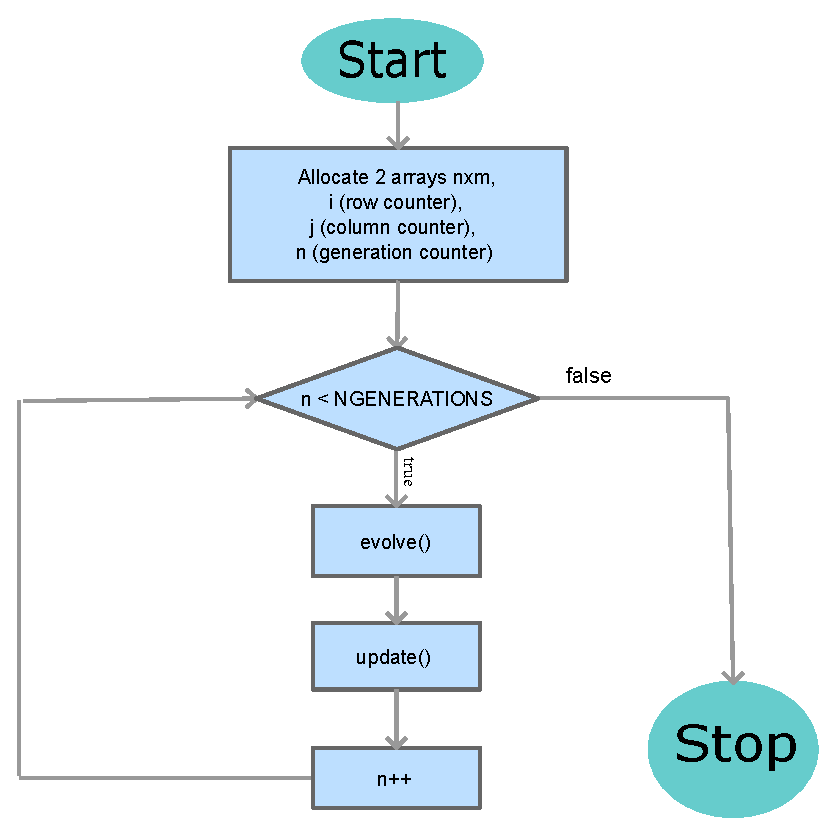
\includegraphics[scale = 0.8]{chart.eps}
	\caption{\emph{Game of Life's flowchart}}\label{fig:1}
\end{figure}

\chapter{Study of available parallelism}

\noindent We studied the available parallelism in all the three functions.

\noindent Looking at the fact that we dealt with a matrix, even if saved as a single array, in every function we had two nested cycles, one to scan rows and another to scan columns. So we thought to parallelize the external cycle in all the functions in order to change more than one row at the same time.

\noindent In our algorithm, there are no complex calculus, the potential speedup is given by the possibility to change more cells at the same time. This is made possible by the fact that there are two matrices that represent the same grid in two different generations, so modifying at the same time the new value of many cells there is not the risk of the result's impairment.
In addition, in the \emph{evolve} function there are two more independent cycles to fix the boundary condition before the evolution of the game. Also these cycles can be parallelized. 
On the contrary, in the \emph{main} routine, the cycle on the generations cannot be parallelized, because one evolution is dependent on the previous one, so it is fundamental to preserve the serial order. 

\chapter{OpenMP parallel implementation}
We thought different parallel implementations:
\begin{enumerate}
\item we tried with one parallel region in every function using static scheduling;
	\item we decided to try opening only one parallel region, at the program start, with the serial cycle on generations and then having the for parallelization on our three functions. We tried this because we thought to avoid the continued creation and destruction of the used thread at each iteration of the generational change. So we expected this version faster than the first. We used static scheduling;
	\item finally we try to use dynamic scheduling with different chunk sizes, instead of the static scheduling, on the version with only one parallel region. We try only on this because we looked that was the quicker.
\end{enumerate}



\chapter{CPU characteristics}
To run the program we used a notebook with as processor Intel® Core™ i5-3230M Processor.
This processor has two physical cores and four logic cores. So, we decided to evaluate the performance of the parallelized code using two and four threads. We expected the best execution was with two threads, but, even if the real core are two, hyper-threading let have some advantage if the instructions are no dependent and so they don't create stalls.

\noindent Our program does not have dependences on the cycles we wanted to parallelize, so it could be that hyper-threading gave benefits even if not so large.

\noindent We report all the CPU's characteristics in Figure \ref{fig:2}.

\begin{figure}
	\centering
	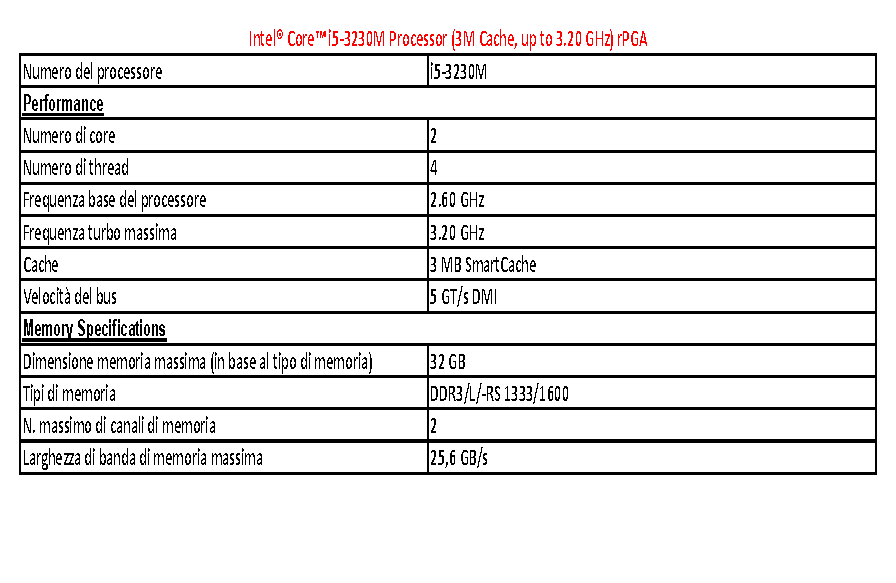
\includegraphics[scale = 0.5]{i5.eps}
	\caption{Processor's characteristics} \label{fig:2}
\end{figure}





\chapter{Performance's Measurements}\label{am}
\noindent Initially we try running the serial program several times, measuring the time interval, using different dimensions of the matrix and different numbers of generations.
We decided to use square matrix to save the times, but we try also some cases with rectangular matrices to see if and how there was changes on the parallel behavior.

\noindent We calculated the theoretical speedup using the Amdahl's law which in the parallelism case affirms that if $f$ is the fraction of a calculus that can be parallelized, $1-f$ is the portion that cannot be parallelized and $N$ is the processor's number and $H(N)$ is the overhead, we can obtain a theoretical speedup of $S_{o} = \frac{1}{(1-f) + \frac{f}{N} + H(N)}$. As seen in \cite{multi}, in case of hyper-threading, the Amdahl's law is different, assuming that every thread goes $\frac{2}{3}$ of the velocity it went without hyper-threading, we find $S_{HT} = \frac{1}{(1-f) + 0,67*(\frac{f}{N}) + H(N)}$ where $N$, now, are the number of logic cores.

\noindent All our functions are parallelized except some assignment that is not significant in term of time spent, so we decided to take $f = 1$. Our processor has two physical cores and so $N =2$, finally using the Amdahl's formula we have $S_o = 2$ assuming $H(N) =0$. While, if we had benefits from multithreading, assuming a overhead of 0.3 more than without hyper-threading, we obtain $S_{HT} = 2.13$.

\noindent Then we measured times of our parallel implementation with different settings. The means of measurements are reported from Figure \ref{fig:4} to Figure \ref{fig:7}, we don't calculate the variance because it is not significant since the results differs only in order of hundredths of a second.

\noindent On x-axis we have the source code used. Specifically, \emph{serial} is the serial version, \emph{parallel1} is the parallel implementation with a parallel region for each function and static scheduling, \emph{parallel2} is the parallel implementation with only one parallel region and static scheduling and \emph{parallel3} is the implementation with one parallel region and dynamic scheduling, so the number after the score is the chunk size used. On y-axis, there are execution's times.


\begin{figure}
	\centering
	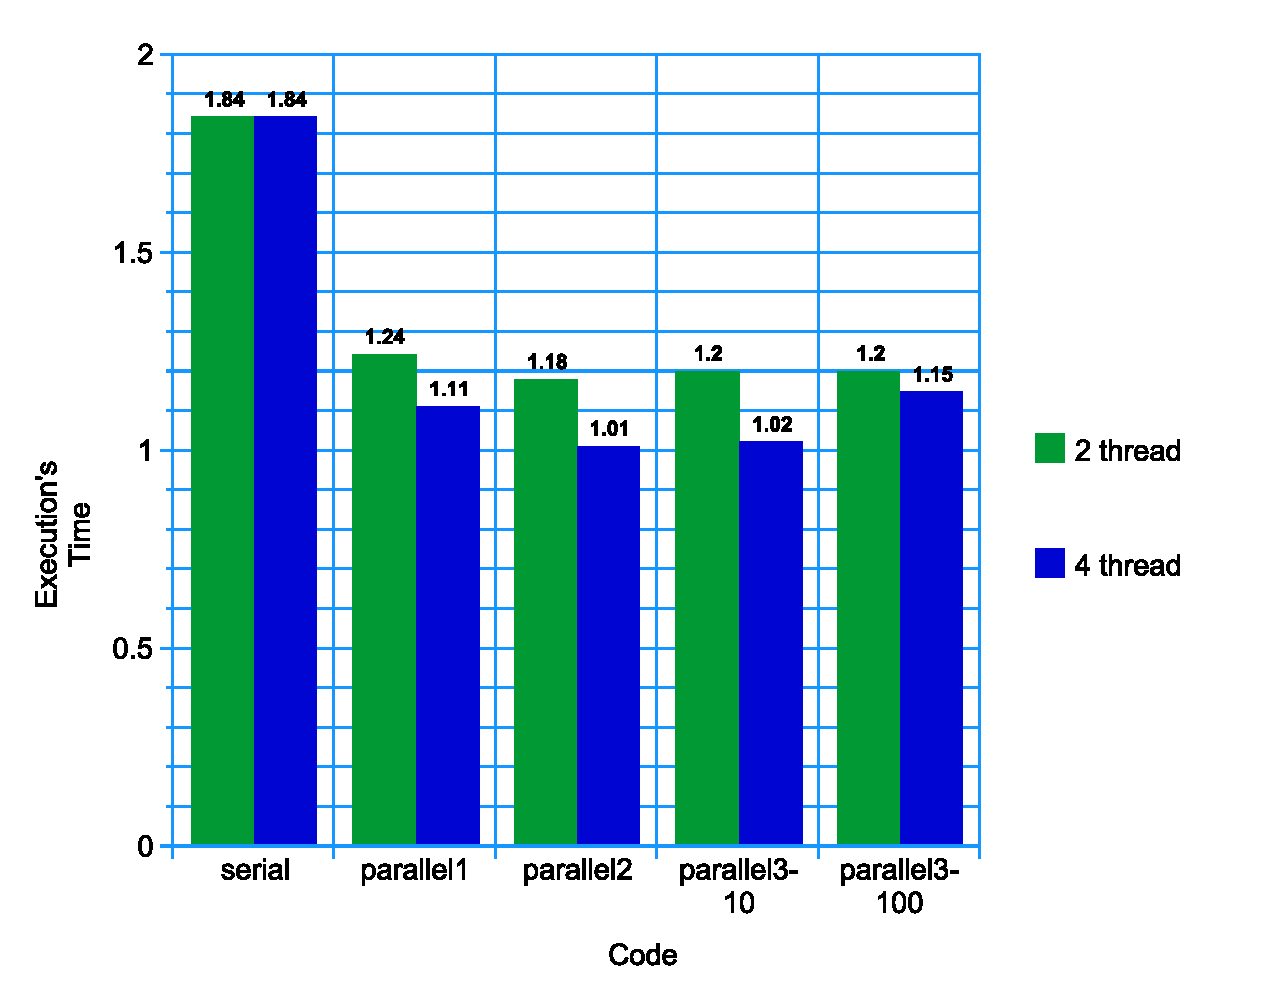
\includegraphics[scale = 0.5]{1000-100.eps}
	\caption{Performances with 100 generations and 1000x1000 matrix} \label{fig:4}
\end{figure}
\begin{figure}
	\centering
	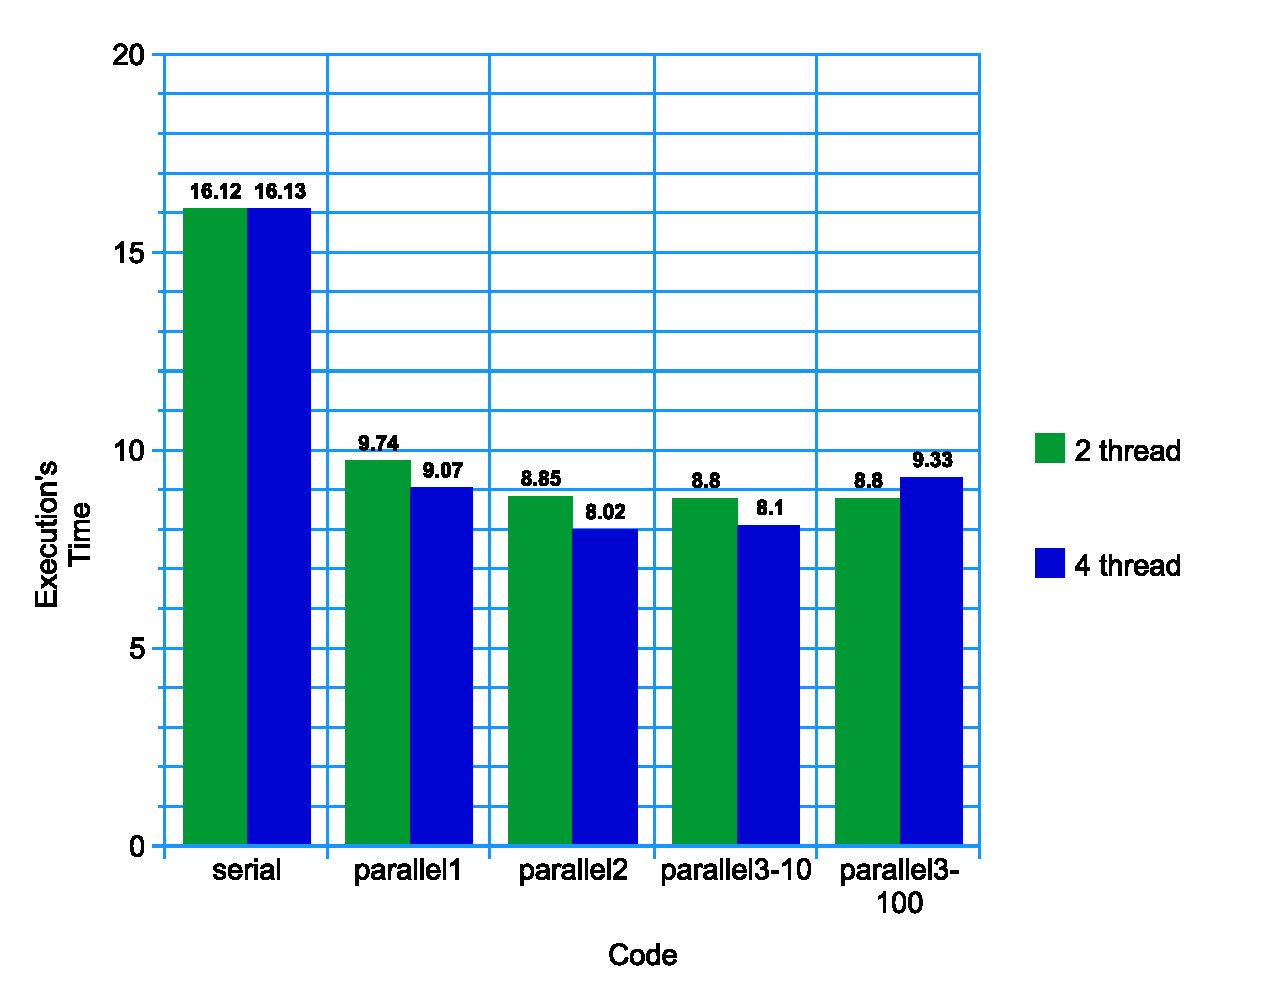
\includegraphics[scale = 0.5]{graph.eps}
	\caption{Performances with 1000 generations and 1000x1000 matrix} \label{fig:3}
\end{figure}
\begin{figure}
	\centering
	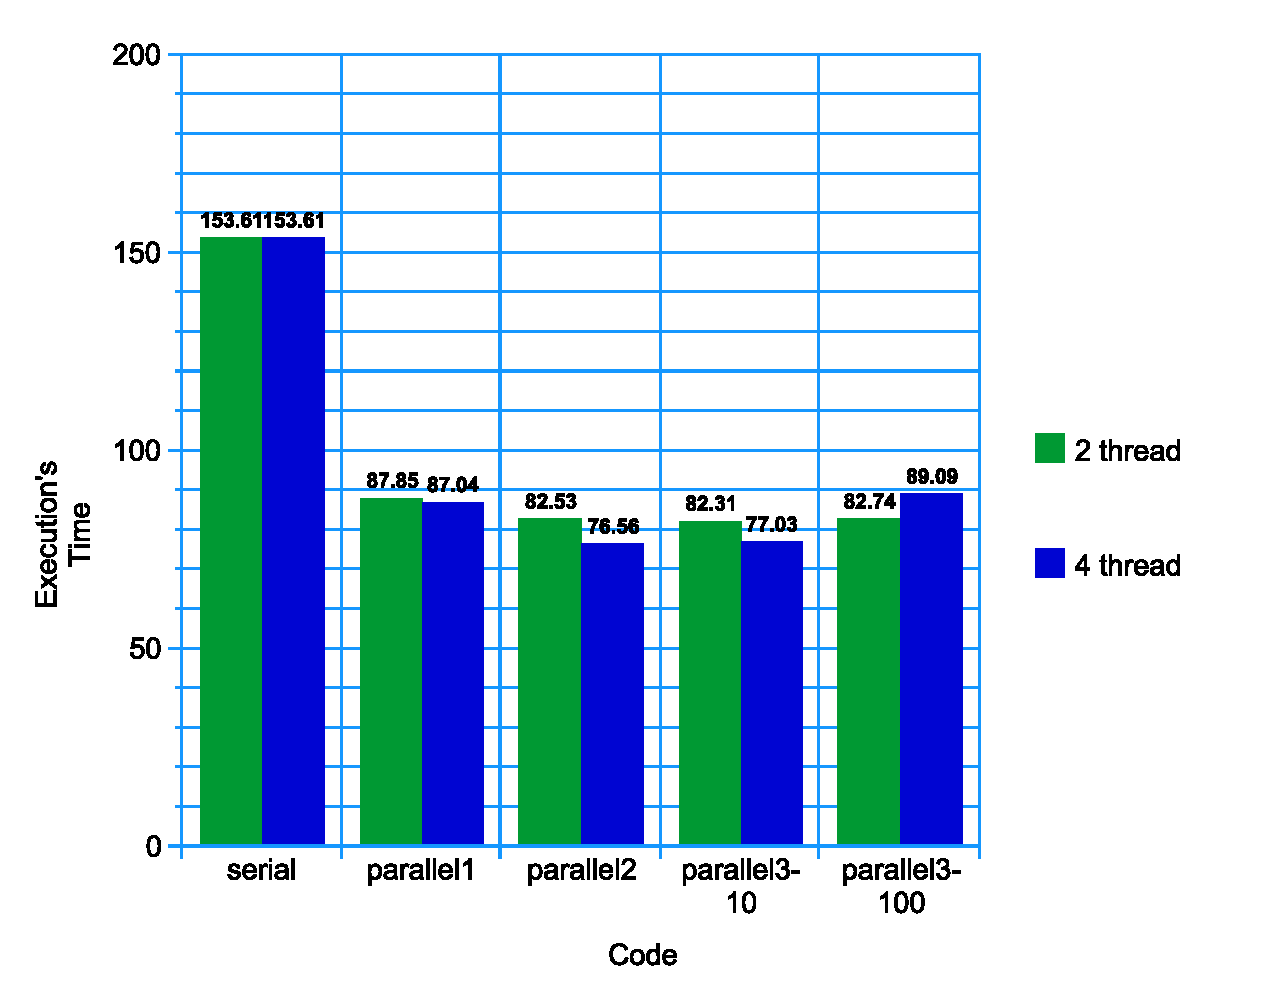
\includegraphics[scale = 0.5]{1000-10000.eps}
	\caption{Performances with 10000 generations and 1000x1000 matrix} \label{fig:5}
\end{figure}
\begin{figure}
	\centering
	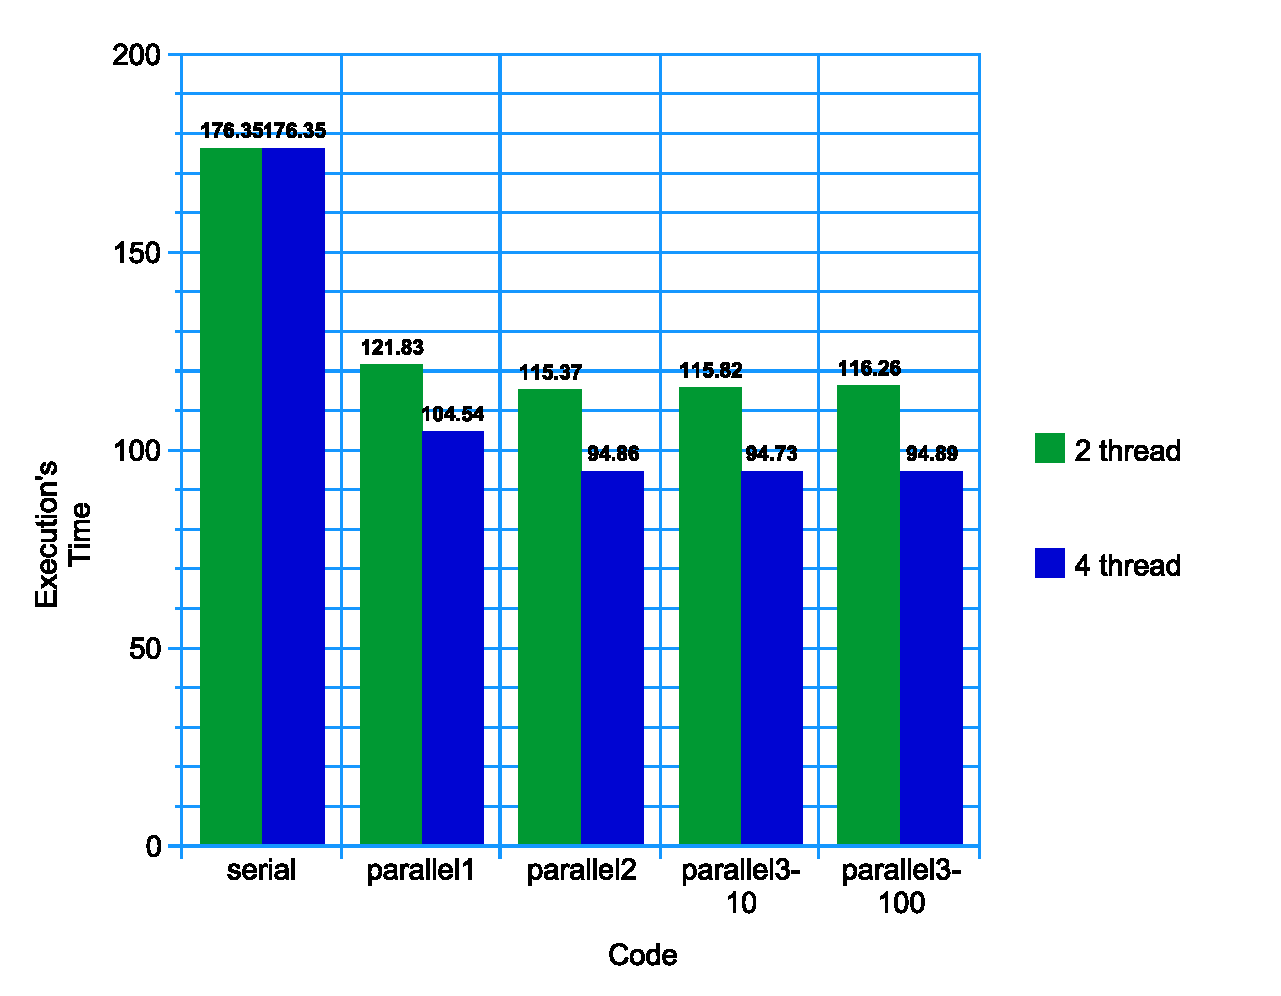
\includegraphics[scale = 0.5]{10000-100.eps}
	\caption{Performances with 100 generations and 10000x10000 matrix} \label{fig:6}
\end{figure}
\begin{figure}
	\centering
	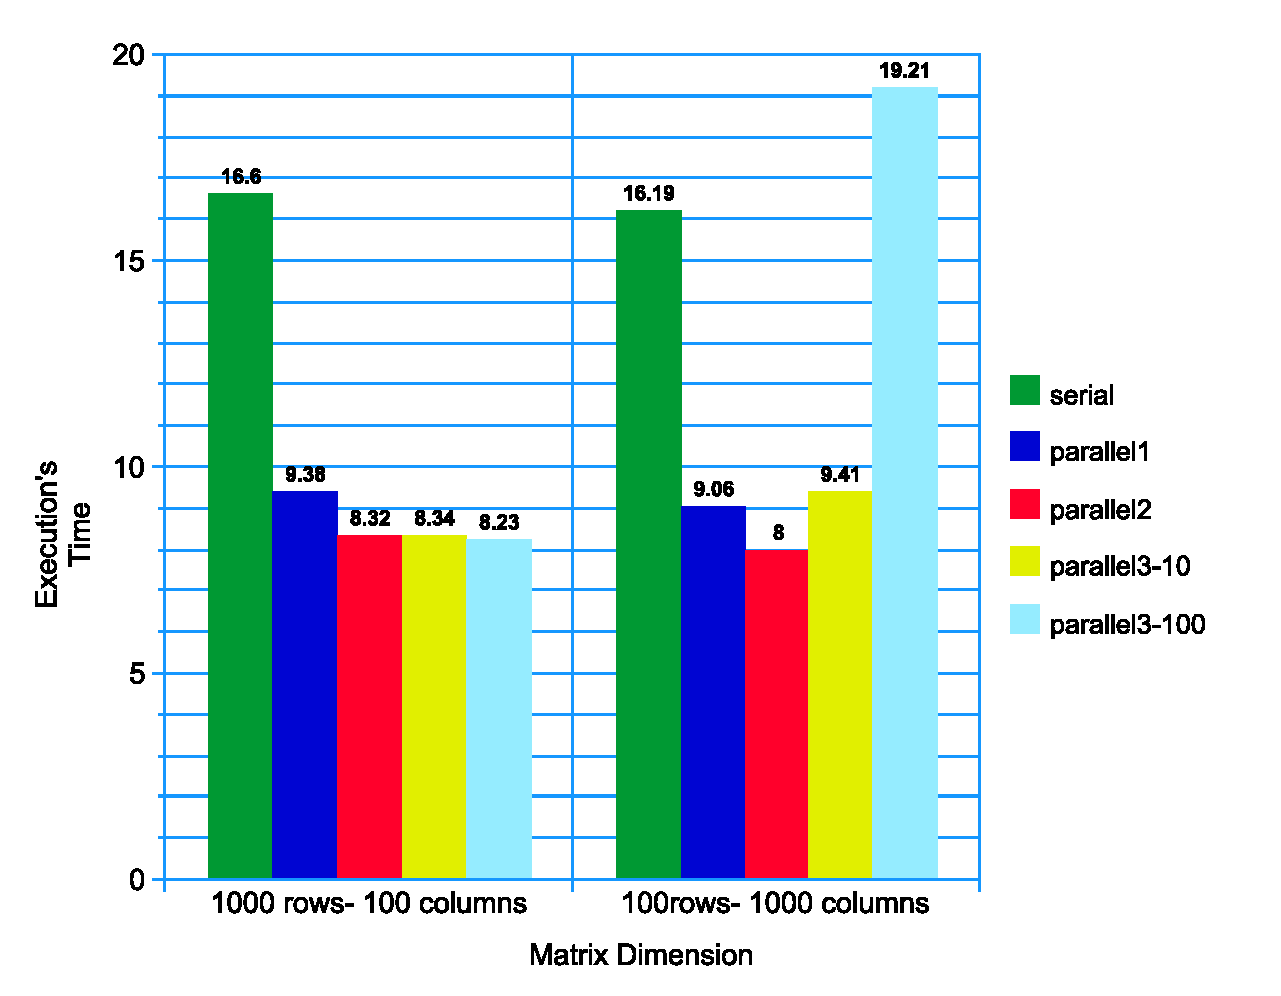
\includegraphics[scale = 0.5]{matdim.eps}
	\caption{Performances with 100 generations and 10000x10000 matrix} \label{fig:7}
\end{figure}

\section{Some Consideration on results}
We can see from Figures that the best version is \emph{parallel2} with four threads in every case. A result not so expected. We expected that \emph{parallel2} was the best, because opening only one parallel region, we spend less time due to creation and destruction of threads in call of functions, but we thought that was better with two threads because we have only two physical CPU's cores. We can explain our results thanks to the particularity of our algorithm, in fact we have neither dependences nor complex calculus, so we benefits of hyper-threading of our processor which permits parallel elaborations on four threads. The benefit is not so high like having four cores, obviously we cannot go over Amdahl result, but we improve the performance of a bit.
We can also look at the performances with dynamic scheduling which become worse as it chunk size grows and it is worse than parallel implementations with static scheduling. This behavior is due to
the algorithm which gives to each thread approximately the same workload, so to force a bigger chunk size means to delete this advantage, charging some thread too much and some other not.
A last consideration concerns with rectangular matrix. Looking at Figure \ref{fig:7} (4 threads) we can see how having a chunk size equal to the number of rows is worse than serial case, in fact only one thread works and there is the waste time due to the creation, destruction of threads and their communication. While it has been the best performance with matrices with 1000 rows which is a multiple of 100 and so it has been a good repartition of the workload.

\section{Speedup}

We can see the speedup for the different simulations with two and four threads in the Figures \ref{fig:8} and \ref{fig:9}. In general, we benefit of parallel programming where the matrix is quite big and there are many generations. If the matrix is small, the serial case is very quick and so the parallelization is unuseful, a too big matrix has to be saved in memory and so there are less parallelization's benefits in term of speedup.

\noindent We can note how \emph{parallel1}, which has more parallel regions, is the worst, in particular the gap is bigger when the number of generations becomes bigger, this behavior was expected. It seems to be better with four threads, but it is only due to the fact that \emph{parallel3-100} has a chunk size very big in relation to matrices dimension we deal with and so it has bad performances on small data, we can see how with a matrix 10000x10000 also \emph{parallel3-100} goes better than \emph{parallel1}. Finally with two threads, except \emph{parallel1}, other implementations have very similar results. With two threads, the maximum speedup obtained is 1.87.
With four threads the maximum speedup is 2.01, a result that cannot be obtained with two threads (the maximum, without overhead, was 2). Being four threads, we obtain similar result with one parallel region with static scheduling or with dynamic scheduling with small chunk size respect to the number of rows to make all threads working.
\begin{center}
\begin{figure}
	\centering
	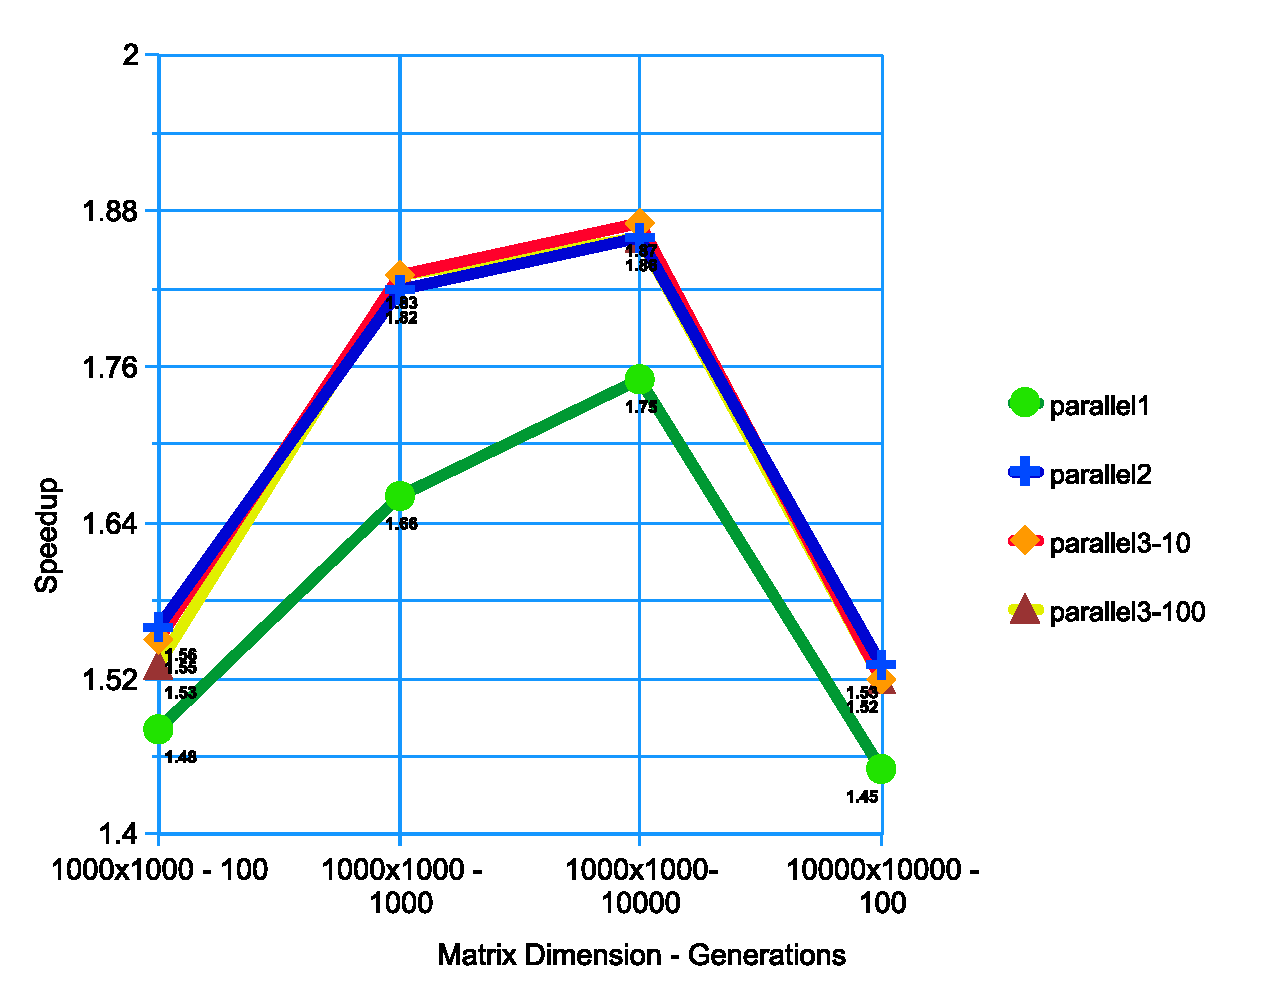
\includegraphics[scale = 0.5]{2.eps}
	\caption{Speedup with two threads} \label{fig:8}
\end{figure}
\end{center}
\begin{center}
\begin{figure}
	\centering
	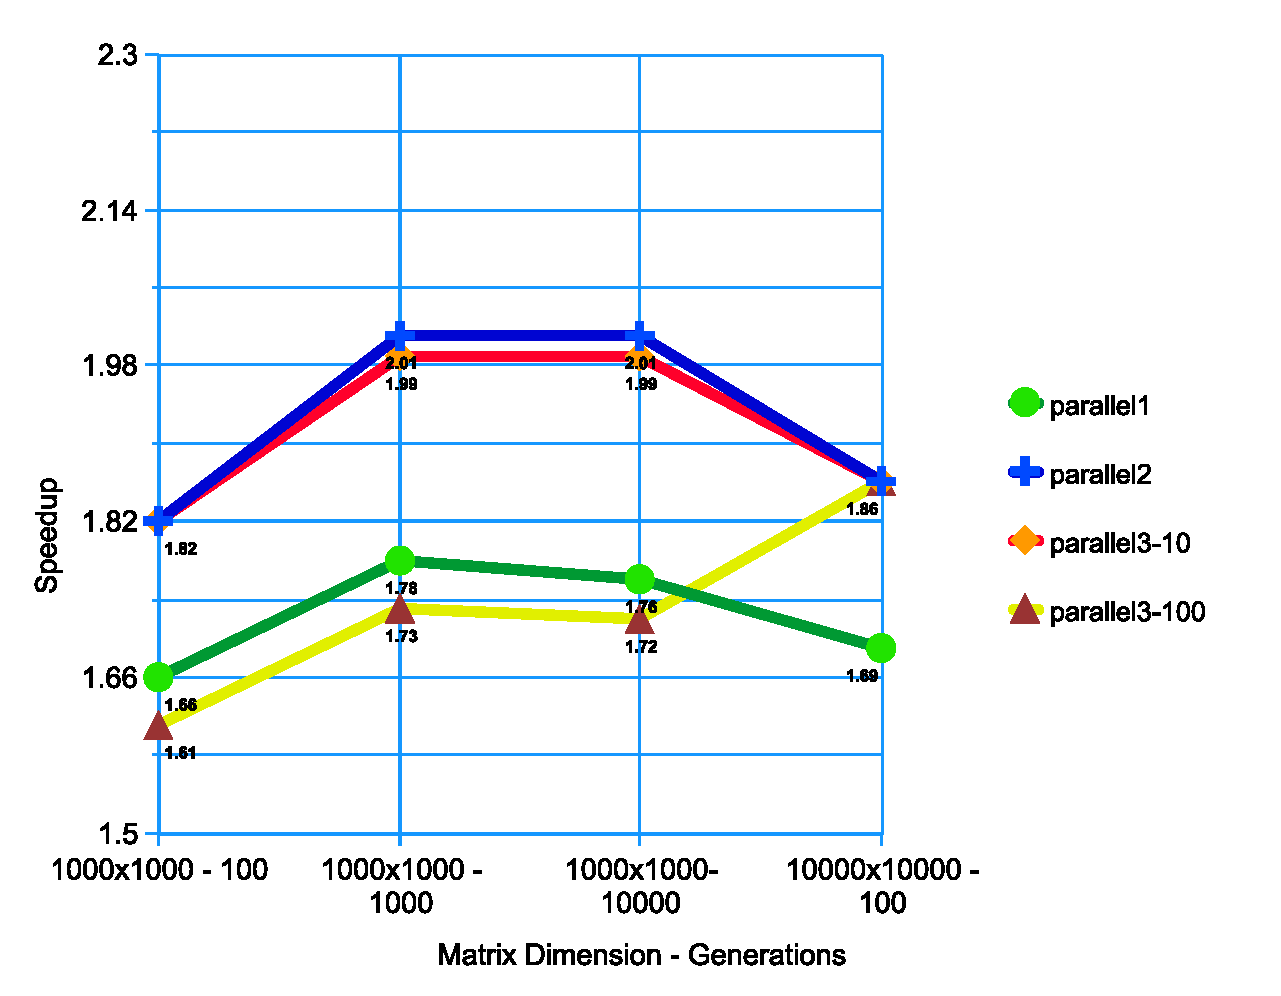
\includegraphics[scale = 0.5]{4.eps}
	\caption{Speedup with four threads} \label{fig:9}
\end{figure}
\end{center}

\chapter{Conclusion}
We start with a serial algorithm without any function and using a matrix, we modified it in three important functions: \emph{init} which initialize the grid, \emph{evolve} which computes the next generation and \emph{update} which change the old generation with the new. We also transformed the matrix into a single array to benefit of the locality of access.

\noindent Then we studied the possible available parallel implementations and we proposed three different implementations:
\begin{enumerate}
\item One with a parallel region in each function and static scheduling;
 \item One with only one parallel region and static scheduling;
 \item One with only one parallel region and dynamic scheduling.
\end{enumerate}
In conclusion we try all the versions with two and four threads using as processor Intel® Core™ i5-3230M Processor and we analyzed the results. We found that the best is the second proposal with four threads. With this, we obtained a maximum speedup of two using a matrix 1000x1000 and with 1000 or more generations. A so high speedup is possible thanks to hyper-threading which has more overhead, but it works with four logic cores, so we have four threads slower than a quad-physical core CPU, but faster than two threads.


\begin{thebibliography}{9}
	\bibitem {Life} Caleb Koch, \emph{Regularity in Conway's Game of Life}, 2015
\bibitem {wiki} Web, \url{https://en.wikipedia.org/wiki/Conway's_Game_of_Life}
\bibitem {stan} Web, \url{http://web.stanford.edu/~cdebs/GameOfLife}
\bibitem {code} Web, \url{https://www.pdc.kth.se/education/tutorials/summer-school/mpi-exercises/mpi-lab-codes/game_of_life-serial.c/view}
\bibitem {multi} Shameem Akhter, Jason Roberts, \emph{Multi-Core Programming, increasing Performance through Software multi-threading}, Intel press pagg.(14-18)
\end{thebibliography}
\end{document}

\end{document}
